\subsection{Anterior à modificação}

O cenário 2 escolhido foi na subestação de Pocinho, à margem do Rio Douro, noroeste de Portugal, retratado na Figura \ref{fig:caso_2_antes_geral_menor}. O cenário será a retirada da linha que liga o gerador de Pocinho à subestação de Pocinho, que atualmente está funcionando com 102\% da sua capacidade de trânsito de potência.

\begin{figure}[H]
	\centering
	\captionsetup{width=\textwidth, font=footnotesize, textfont=bf}	
	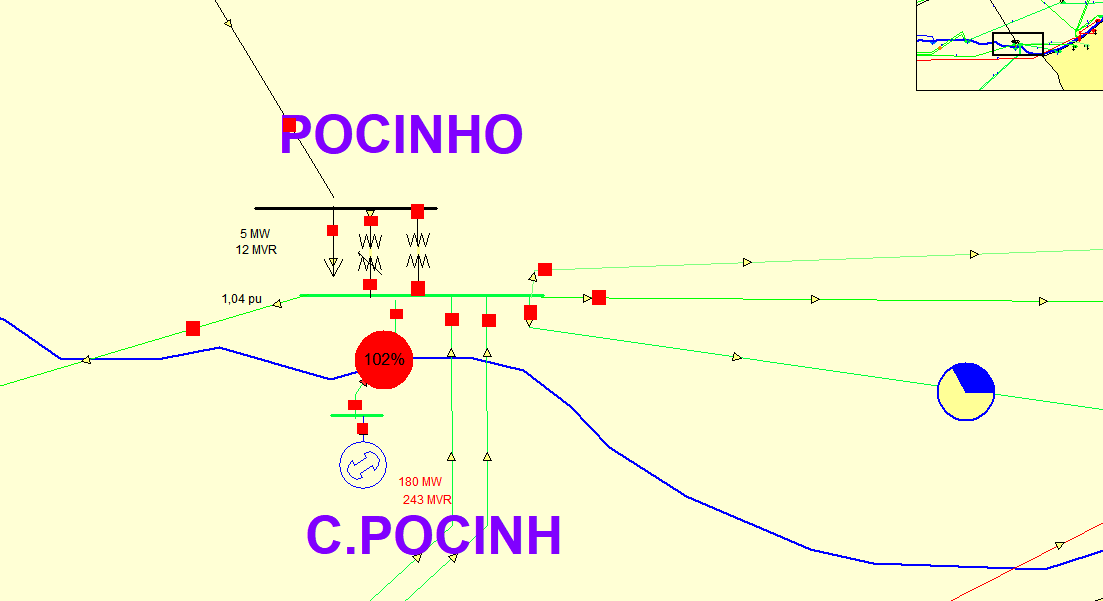
\includegraphics[width=\linewidth]{img/caso_2_antes_geral.PNG}
	\caption{Cenário 2, anterior à modificação}
	\vspace{-3.5mm}
	\caption*{Fonte: autoria própria}
	\label{fig:caso_2_antes_geral_menor}
\end{figure}

Os barramentos que estão diretamente ligados ao barramento (subestação) de Pocinho, circulada em vermelho na Figura \ref{fig:caso_2_antes_geral}, são: M. Cavale, Armamar, Chafariz, Saucelle (Espanha), 489 (Espanha) e Aldeadav (Espanha); todas estas subestações ligadas a Pocinho estão circuladas em azul na Figura \ref{fig:caso_2_antes_geral}.

\begin{figure}[H]
	\centering
	\captionsetup{width=\textwidth, font=footnotesize, textfont=bf}	
	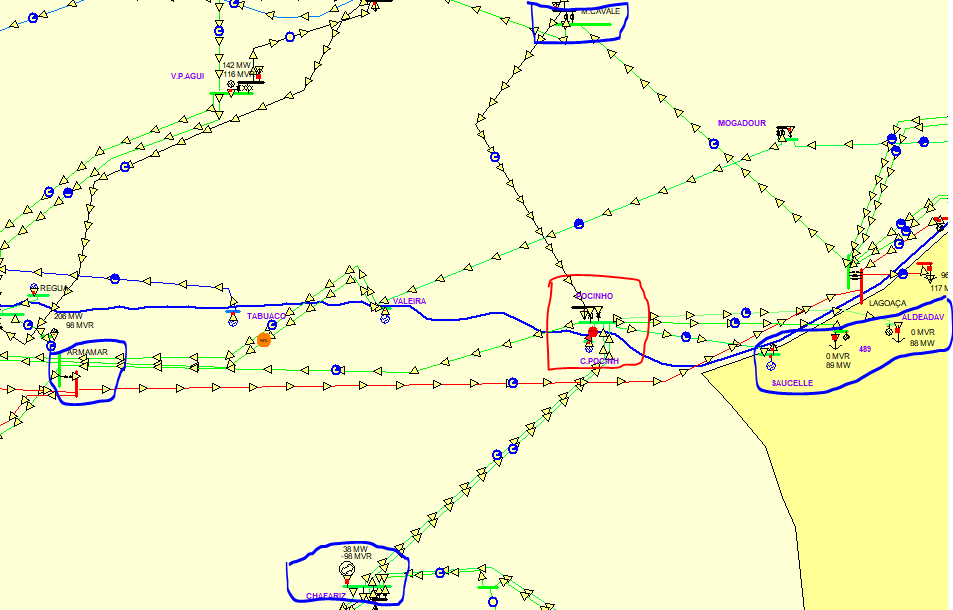
\includegraphics[width=\linewidth]{img/caso_2_antes_expandido.PNG}
	\caption{Vista ampliada do cenário 2, anterior à modificação}
	\vspace{-3.5mm}
	\caption*{Fonte: autoria própria}
	\label{fig:caso_2_antes_geral}
\end{figure}

Os dados globais antes da modificação são os mesmos do caso 1, como pode ser visto na Tabela \ref{tab:DadosGeraisIniciais}. Na Tabela \ref{tab:caso_2_antes} são descritos os valores de geração de potência ativa e reativa do gerador de Pocinho, carregamento das linhas em conexão com a subestação de Pocinho, módulo e ângulo dos barramentos ligados a Pocinho, potência ativa e reativa líquida entre Portugal e Espanha na região próxima a Pocinho, bem como o sentido do fluxo de potência nas linhas.

\begin{table}[H]
\centering
\small
\captionsetup{width=.76\textwidth, font=footnotesize, textfont=bf}
\begin{tabular}{llcc}
\multicolumn{4}{c}{\cellcolor[HTML]{333333}{\color[HTML]{FFFFFF} \textbf{Carregamento das linhas}}} \\
 & \multicolumn{1}{c}{\textbf{Sentido da Potência}} &  & \textbf{Carregamento (\%)} \\
\textbf{Pocinho} & \multicolumn{1}{c}{$<-$} & \multicolumn{1}{l}{\textbf{M. Cavale}} & 2 \\
\textbf{Pocinho} & \multicolumn{1}{c}{$->$} & \multicolumn{1}{l}{\textbf{Armamar}} & 17,3 \\
\textbf{Pocinho} & \multicolumn{1}{c}{$<-$} & \multicolumn{1}{l}{\textbf{Chafariz}} & 6 \\
\textbf{Pocinho} & \multicolumn{1}{c}{$->$} & \multicolumn{1}{l}{\textbf{Saucelle}} & 32,9 \\
\textbf{Pocinho} & \multicolumn{1}{c}{$->$} & \multicolumn{1}{l}{\textbf{489}} & 29,6 \\
\textbf{Pocinho} & \multicolumn{1}{c}{$->$} & \multicolumn{1}{l}{\textbf{Aldedav}} & 29,2 \\
\multicolumn{4}{c}{\cellcolor[HTML]{333333}{\color[HTML]{FFFFFF} \textbf{Tensão nas barras}}} \\
 &  & \textbf{Módulo} & \textbf{Ângulo} \\
\cellcolor[HTML]{036400}{\color[HTML]{FFFFFF} } & \textbf{Pocinho} & 1,0376 & 32,275 \\
\cellcolor[HTML]{036400}{\color[HTML]{FFFFFF} } & \textbf{M. Cavale} & 1,0493 & 33,348 \\
\cellcolor[HTML]{036400}{\color[HTML]{FFFFFF} } & \textbf{Armamar} & 1,0484 & 28,552 \\
\multirow{-4}{*}{\cellcolor[HTML]{036400}{\color[HTML]{FFFFFF} \textbf{Portugal}}} & \textbf{Chafariz} & 1,04 & 32,932 \\
\multicolumn{1}{c}{\cellcolor[HTML]{CD9934}{\color[HTML]{FFFFFF} \textbf{}}} & \textbf{Saucelle} & 1 & 32,206 \\
\cellcolor[HTML]{CD9934}{\color[HTML]{FFFFFF} \textbf{Espannha}} & \textbf{489} & 1 & 30,837 \\
\cellcolor[HTML]{CD9934}{\color[HTML]{FFFFFF} } & \textbf{Aldeadav} & 1 & 30,832 \\
\multicolumn{4}{c}{\cellcolor[HTML]{333333}{\color[HTML]{FFFFFF} \textbf{Geradores}}} \\
 &  & \textbf{MW} & \textbf{MVar} \\
\multicolumn{1}{c}{\cellcolor[HTML]{036400}{\color[HTML]{FFFFFF} }} & \textbf{Pocinho} & 180 & 243 \\
\multicolumn{1}{c}{\multirow{-2}{*}{\cellcolor[HTML]{036400}{\color[HTML]{FFFFFF} \textbf{Portugal}}}} & \textbf{Chafariz} & 38 & -98 \\
\cellcolor[HTML]{CD9934}{\color[HTML]{FFFFFF} } & \textbf{Saucelle} & 0 & -137 \\
\cellcolor[HTML]{CD9934}{\color[HTML]{FFFFFF} \textbf{Espannha}} & \textbf{489} & 0 & -92 \\
\cellcolor[HTML]{CD9934}{\color[HTML]{FFFFFF} } & \textbf{Aldeadav} & 0 & -91 \\
\multicolumn{4}{c}{\cellcolor[HTML]{333333}{\color[HTML]{FFFFFF} \textbf{Interligação com Espanha}}} \\
\multicolumn{2}{l}{\textbf{Portugal $->$ Espanha}} & 208,9 MW & 320,5 MVAr\\
\hline
\end{tabular}
  \caption{Dados iniciais para o caso 2}
  \vspace{-3.5mm}
	\caption*{Fonte: Autoria Própria}
  \label{tab:caso_2_antes}
\end{table}

% - sUBSECTION
\subsection{Análise do impacto da modificação}
Realizando a modificação, abertura da linha que liga o gerador de Pocinho à subestação de Pocinho, conforme a Figura \ref{fig:caso_2_depois_geral_menor} e com vista ampliado na Figura \ref{fig:caso_2_depois_geral}. Na Tabela \ref{tab:caso_2_depois} são descritos os valores para análise após a modificação do caso 2.

\begin{figure}[H]
	\centering
	\captionsetup{width=\textwidth, font=footnotesize, textfont=bf}	
	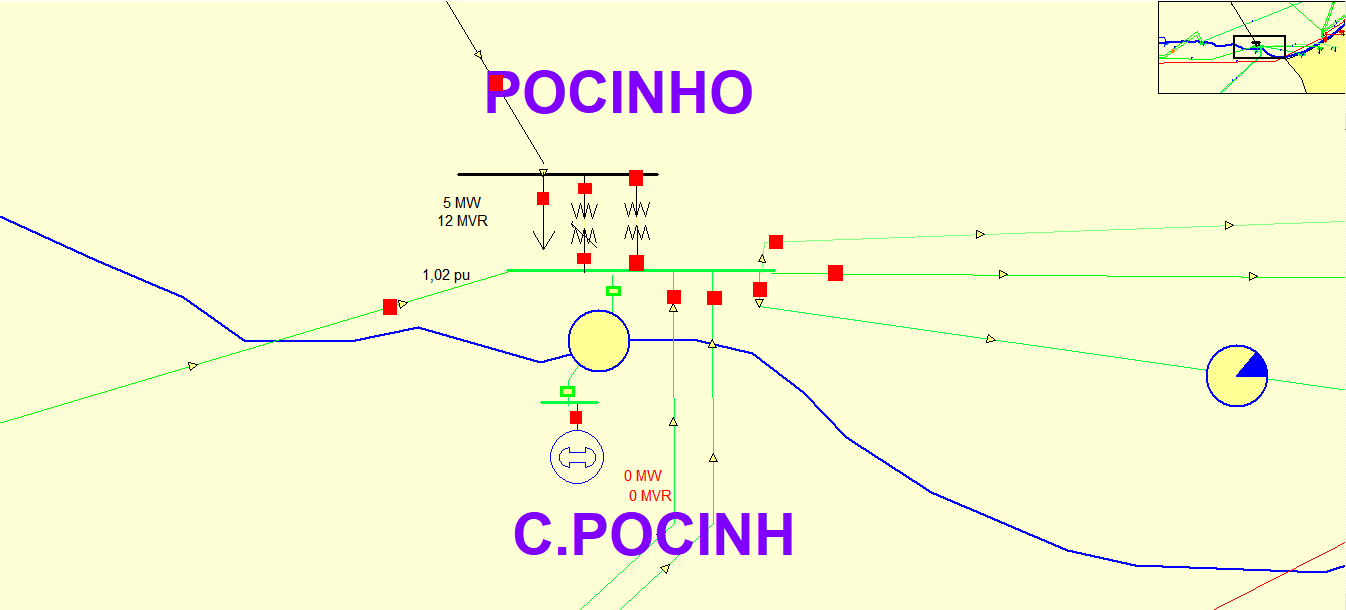
\includegraphics[width=\linewidth]{img/caso_2_depois_geral.PNG}
	\caption{Cenário 2, após a modificação}
	\vspace{-3.5mm}
	\caption*{Fonte: autoria própria}
	\label{fig:caso_2_depois_geral_menor}
\end{figure}

\begin{figure}[H]
	\centering
	\captionsetup{width=\textwidth, font=footnotesize, textfont=bf}	
	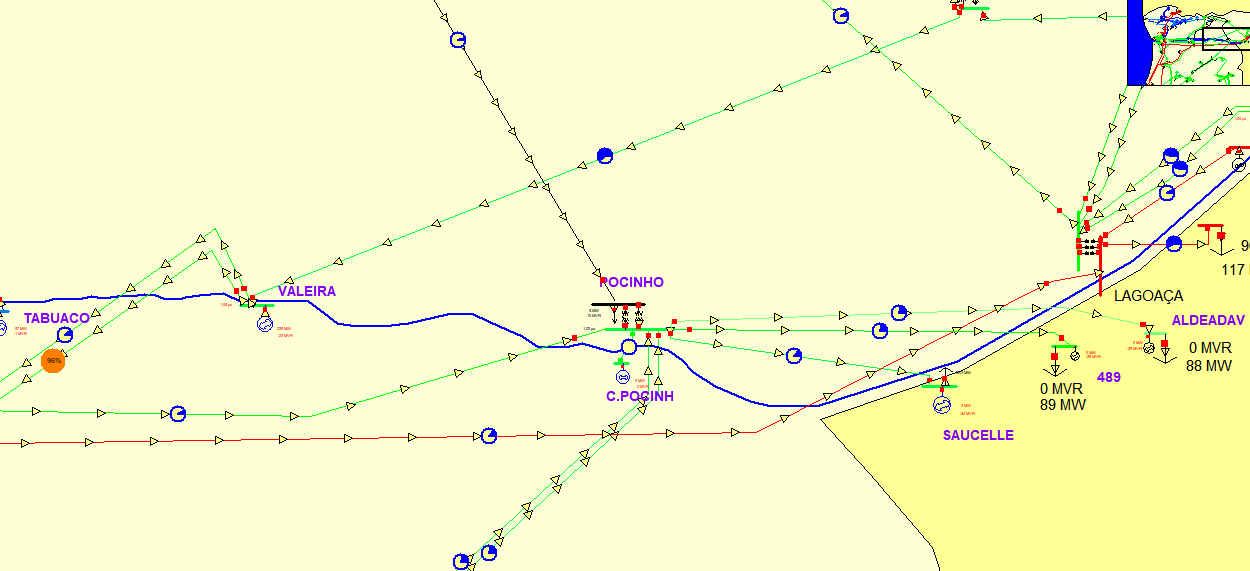
\includegraphics[width=\linewidth]{img/caso_2_depois_expandido.PNG}
	\caption{Vista ampliada do cenário 2, após a modificação}
	\vspace{-3.5mm}
	\caption*{Fonte: autoria própria}
	\label{fig:caso_2_depois_geral}
\end{figure}

\begin{table}[H]
\centering
\small
\captionsetup{width=.76\textwidth, font=footnotesize, textfont=bf}
\begin{tabular}{llcc}
\multicolumn{4}{c}{\cellcolor[HTML]{333333}{\color[HTML]{FFFFFF} \textbf{Carregamento das linhas}}} \\
 & \multicolumn{1}{c}{\textbf{Sentido da Potência}} &  & \textbf{Carregamento (\%)} \\
\textbf{Pocinho} & \multicolumn{1}{c}{$<-$} & \multicolumn{1}{l}{\textbf{M. Cavale}} & 4,3 \\
\textbf{Pocinho} & \multicolumn{1}{c}{$<-$} & \multicolumn{1}{l}{\textbf{Armamar}} & 9 \\
\textbf{Pocinho} & \multicolumn{1}{c}{$<-$} & \multicolumn{1}{l}{\textbf{Chafariz}} & 21,8 \\
\textbf{Pocinho} & \multicolumn{1}{c}{$->$} & \multicolumn{1}{l}{\textbf{Saucelle}} & 13,8 \\
\textbf{Pocinho} & \multicolumn{1}{c}{$->$} & \multicolumn{1}{l}{\textbf{489}} & 21,5 \\
\textbf{Pocinho} & \multicolumn{1}{c}{$->$} & \multicolumn{1}{l}{\textbf{Aldedav}} & 21,2 \\
\multicolumn{4}{c}{\cellcolor[HTML]{333333}{\color[HTML]{FFFFFF} \textbf{Tensão nas barras}}} \\
 &  & \textbf{Módulo} & \textbf{Ângulo} \\
\cellcolor[HTML]{036400}{\color[HTML]{FFFFFF} } & \textbf{Pocinho} & 1,0155 & 25,644 \\
\cellcolor[HTML]{036400}{\color[HTML]{FFFFFF} } & \textbf{M. Cavale} & 1,0384 & 28,661 \\
\cellcolor[HTML]{036400}{\color[HTML]{FFFFFF} } & \textbf{Armamar} & 1,0498 & 25,102 \\
\multirow{-4}{*}{\cellcolor[HTML]{036400}{\color[HTML]{FFFFFF} \textbf{Portugal}}} & \textbf{Chafariz} & 1,0400 & 27,690 \\
\multicolumn{1}{c}{\cellcolor[HTML]{CD9934}{\color[HTML]{FFFFFF} \textbf{}}} & \textbf{Saucelle} & 1 & 25,349 \\
\cellcolor[HTML]{CD9934}{\color[HTML]{FFFFFF} \textbf{Espannha}} & \textbf{489} & 1 & 23,953 \\
\cellcolor[HTML]{CD9934}{\color[HTML]{FFFFFF} } & \textbf{Aldeadav} & 1 & 23,950 \\
\multicolumn{4}{c}{\cellcolor[HTML]{333333}{\color[HTML]{FFFFFF} \textbf{Geradores}}} \\
 &  & \textbf{MW} & \textbf{MVar} \\
\multicolumn{1}{c}{\cellcolor[HTML]{036400}{\color[HTML]{FFFFFF} }} & \textbf{Pocinho} & 0 & 0 \\
\multicolumn{1}{c}{\multirow{-2}{*}{\cellcolor[HTML]{036400}{\color[HTML]{FFFFFF} \textbf{Portugal}}}} & \textbf{Chafariz} & 38 & -18 \\
\cellcolor[HTML]{CD9934}{\color[HTML]{FFFFFF} } & \textbf{Saucelle} & 0 & -54 \\
\cellcolor[HTML]{CD9934}{\color[HTML]{FFFFFF} \textbf{Espannha}} & \textbf{489} & 0 & -29 \\
\cellcolor[HTML]{CD9934}{\color[HTML]{FFFFFF} } & \textbf{Aldeadav} & 0 & -29 \\
\multicolumn{4}{c}{\cellcolor[HTML]{333333}{\color[HTML]{FFFFFF} \textbf{Interligação com Espanha}}} \\
\multicolumn{2}{l}{\textbf{Portugal $->$ Espanha}} & 207,2 MW & 104,8 MVAr\\
\hline
\end{tabular}
  \caption{Dados após modificação para o caso 2}
  \vspace{-3.5mm}
	\caption*{Fonte: Autoria Própria}
  \label{tab:caso_2_depois}
\end{table}

Inicialmente é possível verificar que a linha entre Pocinho e Armamar alterou o sentido do fluxo de potência. Isso pode ser explicado pelo facto que o gerador de Pocinho estava a enviar potência para a interligação com a Espanha e ainda alimentava Armamar; com a sua retirada, houve necessidade de alimentar a interligação com a Espanha com potência ativa de outros geradores, como as outras linhas em contacto com Pocinho já estavam no sentido de enviar potência para ela, ficou apenas a linha com Armamar a alterar o sentido. Os dados globais do sistema após a modificação estão mostrados na Tabela \ref{tab:DadosGerais_caso_2}. A seguir irá ser analisado com mais detalhes os impactos do caso em estudo.

\begin{table}[H]
\centering
	\captionsetup{width=0.4\textwidth, font=footnotesize, textfont=bf}
    \begin{tabular}{|
  >{\columncolor[HTML]{000000}}l |c|c|l}
  \cline{1-3}
  {\color[HTML]{FFFFFF} } & \cellcolor[HTML]{000000}{\color[HTML]{FFFFFF} MW} & \cellcolor[HTML]{000000}{\color[HTML]{FFFFFF} MVAr} &  \\ \cline{1-3}
  {\color[HTML]{FFFFFF} Perdas}  & 207,58 & -568,00  &  \\ \cline{1-3}
  {\color[HTML]{FFFFFF} Geração} & 6772,1 & -504,4  &  \\ \cline{1-3}
  {\color[HTML]{FFFFFF} Cargas}  & 6564,5 & 1814,2 &  \\ \cline{1-3}
  \end{tabular}
  \caption{Dados gerais após caso 2}
  \vspace{-3.5mm}
	\caption*{Fonte: Autoria Própria}
  \label{tab:DadosGerais_caso_2}
\end{table}

\subsubsection{Análise global}
Os impactos da modificação na análise global estão resumidos no gráfico da Figura \ref{fig:global_MW_caso2} para a potência ativa e na Figura \ref{fig:global_MVAr_caso2} para a potência reativa.

\begin{figure}[H]
	\centering
	\captionsetup{width=\textwidth, font=footnotesize, textfont=bf}	
	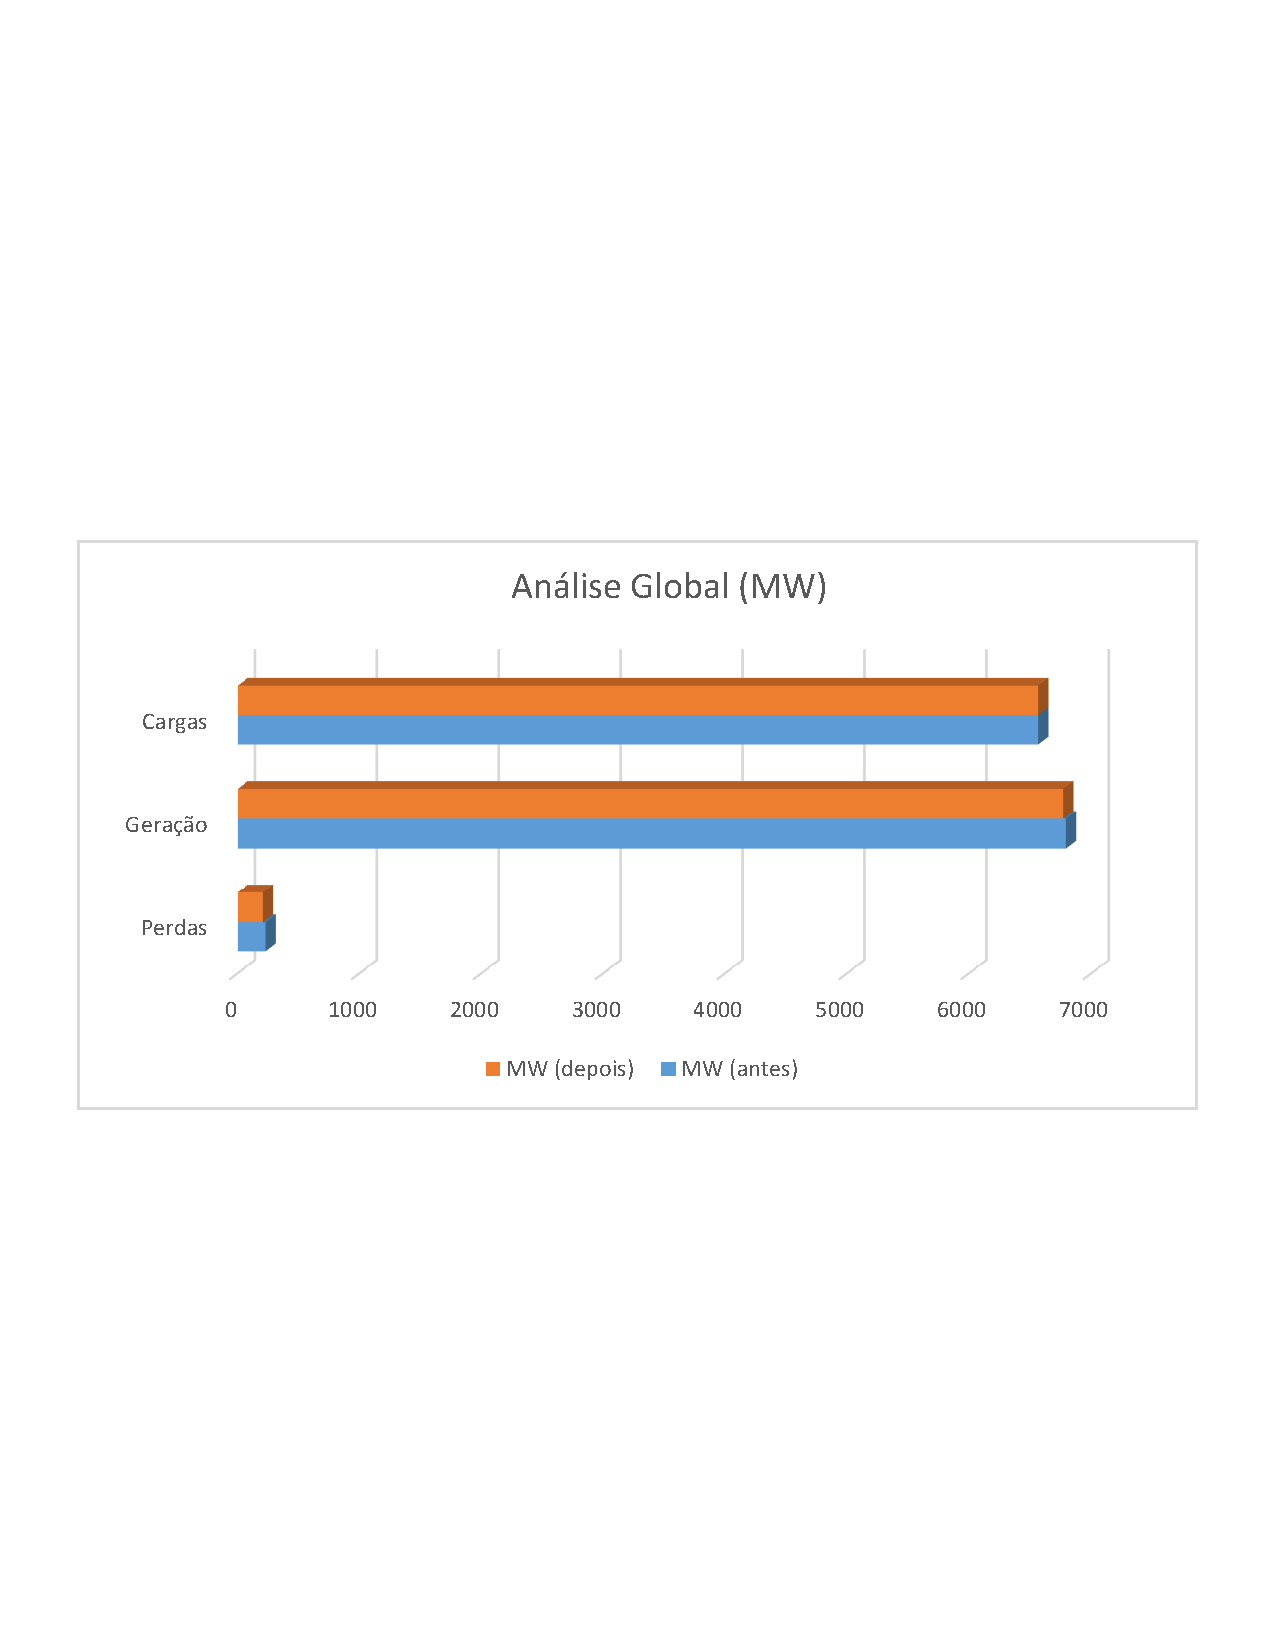
\includegraphics[width=\linewidth,trim = 20mm 97mm 20mm 105mm,clip]{img/global_MW_caso2.pdf}
	\caption{Análise ativa global antes e após o cenário 2}
	\vspace{-3.5mm}
	\caption*{Fonte: autoria própria}
	\label{fig:global_MW_caso2}
\end{figure}

Pelas Figuras \ref{fig:global_MW_caso2} e \ref{fig:global_MVAr_caso2} é atestado que as cargas não variaram, o que mostra que apenas foi retirado geração. Um facto interessante é que as perdas ativas globais diminuíram, isso pode ser explicado porque as linhas que aumentaram o carregamento foram as linhas Pocinho - Chafariz e Pocinho - M. Cavale, sendo que a Pocinho - Chafariz passou de 6\% para 21,8\% de carregamento, conforme Figura \ref{fig:carregamento_linhas_caso2}. 

\begin{figure}[H]
	\centering
	\captionsetup{width=\textwidth, font=footnotesize, textfont=bf}	
	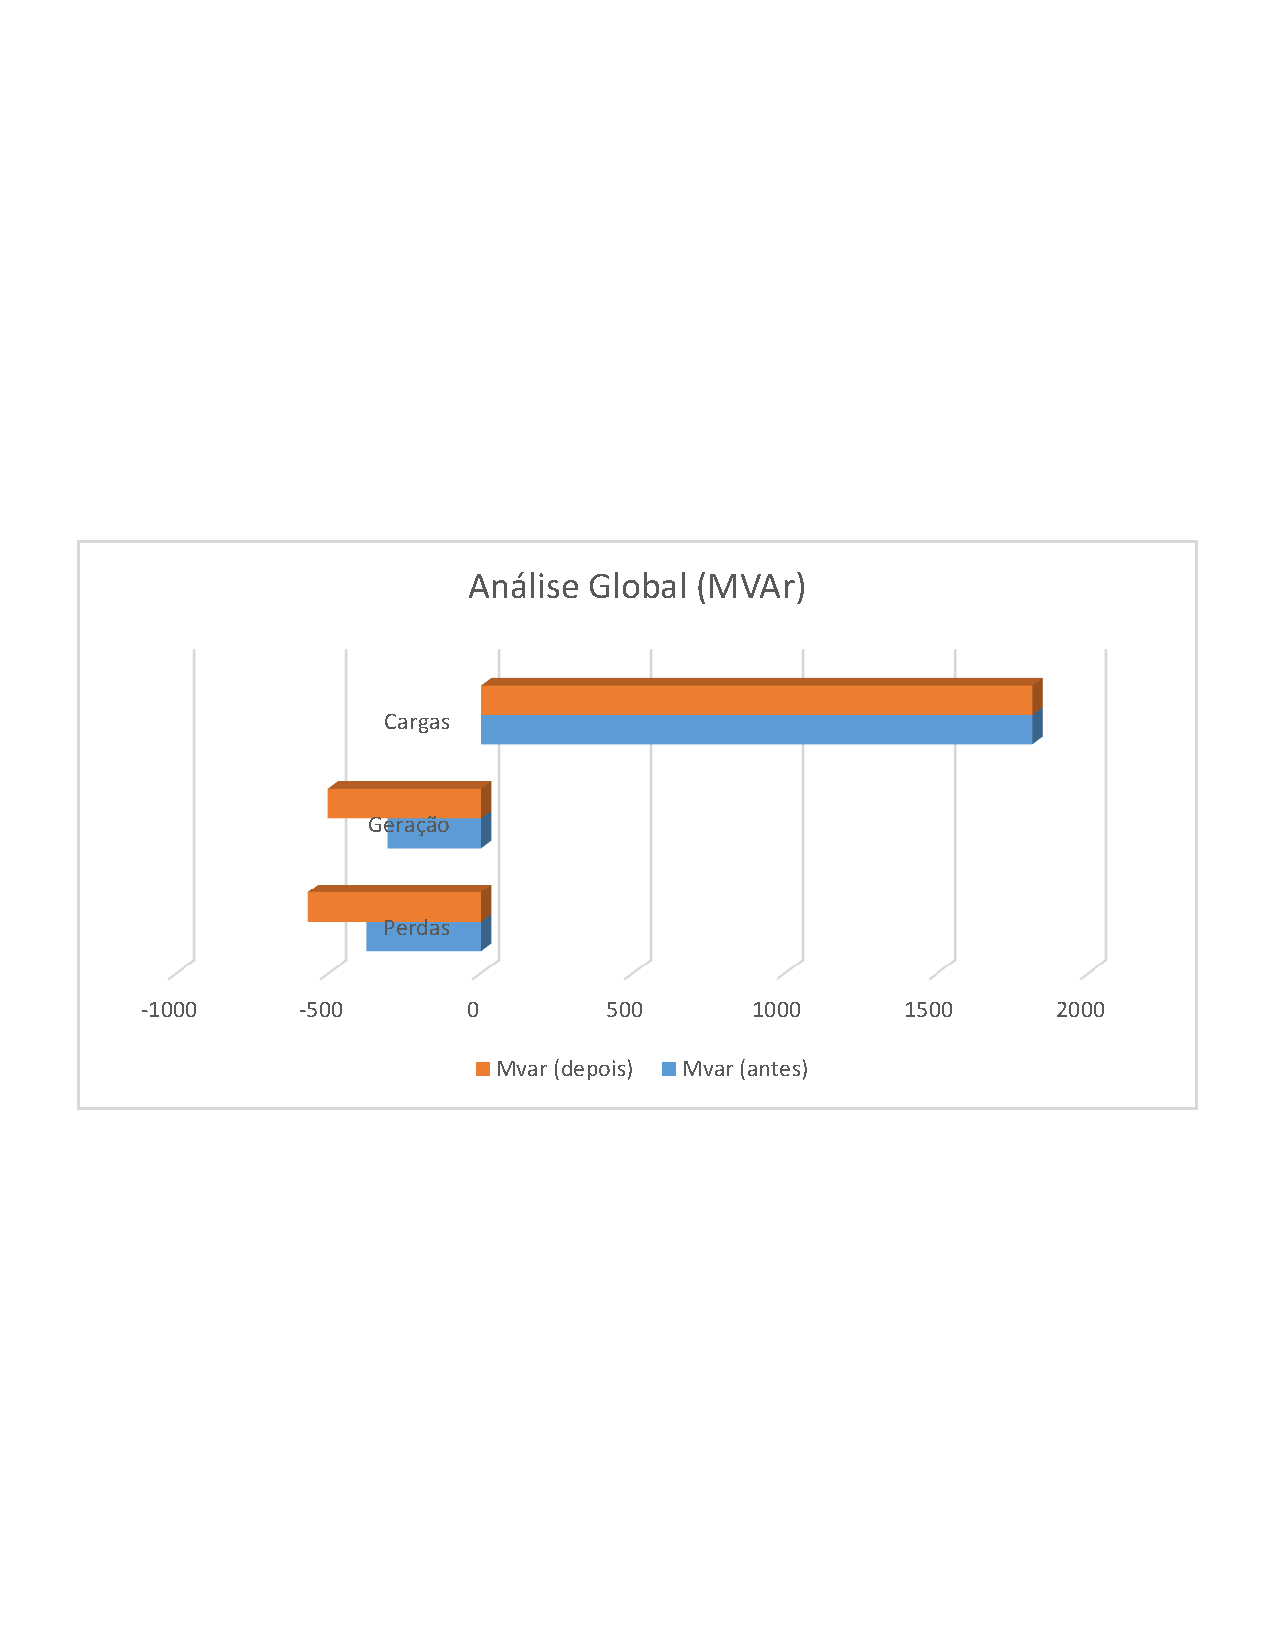
\includegraphics[width=\linewidth,trim = 20mm 97mm 20mm 105mm,clip]{img/global_MVAr_caso2.pdf}
	\caption{Análise reativa global antes e após o cenário 2}
	\vspace{-3.5mm}
	\caption*{Fonte: autoria própria}
	\label{fig:global_MVAr_caso2}
\end{figure}

Observando o gráfico da Figura \ref{fig:global_MVAr_caso2} é visto que houve maior produção de potência reativa capacitiva a fim de atender a também elevação das potência reativa capacitiva das perdas, estas devido ao aumento de carregamento das linhas, o que ocasiona maior efeito capacitivo nas linhas de transmissão.

\subsubsection{Analisar geradores}
O impacto da modificação nos geradores dos barramentos próximos estão resumidas no gráfico da Figura \ref{fig:geradores_caso2}. É evidente a saída da contribuição do gerador de Pocinho, outro facto evidente é a redução da geração de potência reativa capacitiva neste grupo de geradores. Tal redução de capacitivo pode ser explicado pelo fato que antes o gerador de Pocinho gerava apenas potência reativa indutiva, com a saída dele, os outros geradores tiveram que gerar menos capacitivo. 

\begin{figure}[H]
	\centering
	\captionsetup{width=\textwidth, font=footnotesize, textfont=bf}	
	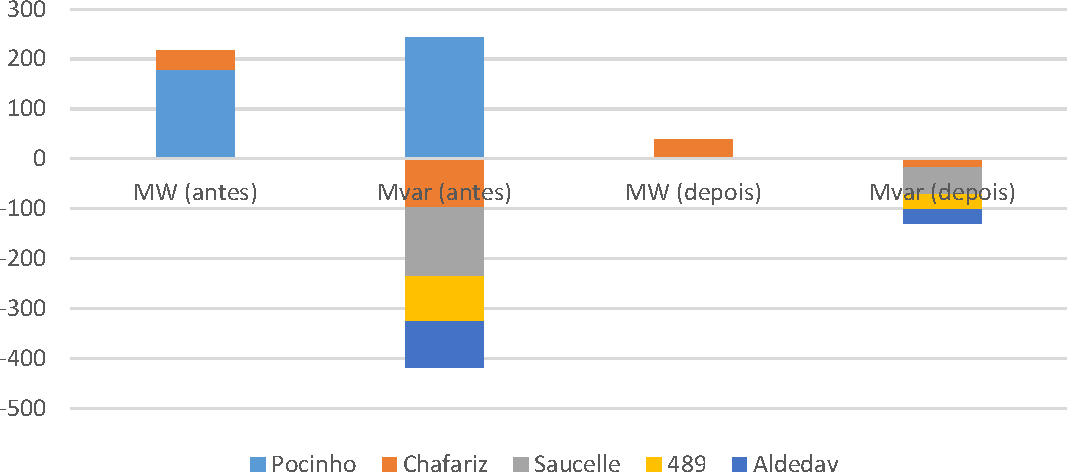
\includegraphics[width=\linewidth]{img/geradores_caso2.pdf}
	\caption{Análise dos geradores antes e após o cenário 2}
	\vspace{-3.5mm}
	\caption*{Fonte: autoria própria}
	\label{fig:geradores_caso2}
\end{figure}

% comentar
\subsubsection{Análise das linhas}
Os impactos da modificação no carregamento das linhas ligadas à subestação de Pocinho estão resumidos no gráfico da Figura \ref{fig:carregamento_linhas_caso2}.

\begin{figure}[H]
	\centering
	\captionsetup{width=\textwidth, font=footnotesize, textfont=bf}	
	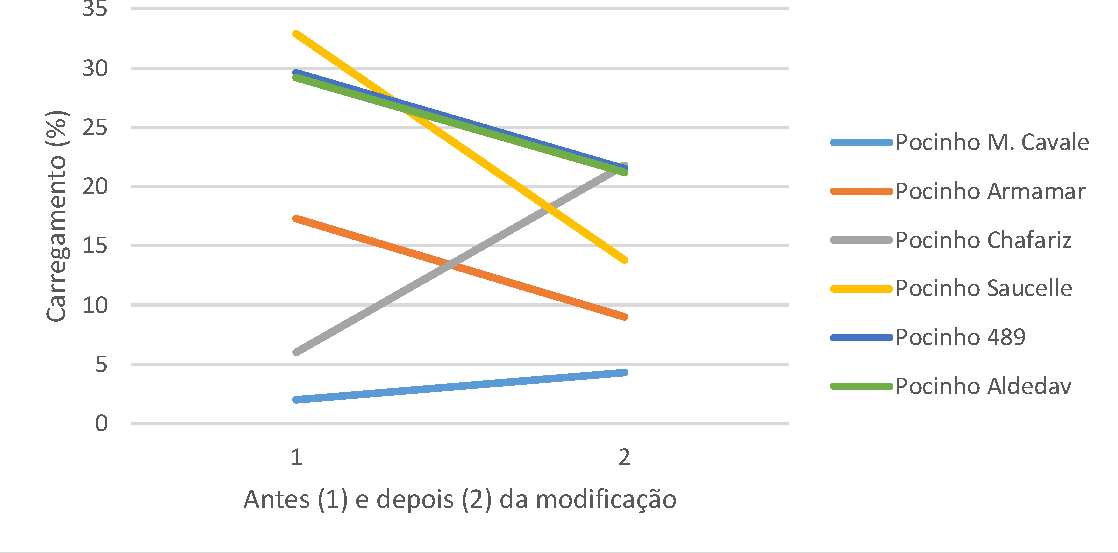
\includegraphics[width=\linewidth]{img/carregamento_linhas_caso2.pdf}
	\caption{Análise do carregamento das linhas antes e após o cenário 2}
	\vspace{-3.5mm}
	\caption*{Fonte: autoria própria}
	\label{fig:carregamento_linhas_caso2}
\end{figure}

	% Mudança do trânsito de potência
	% Sobrecargas

% comentar
\subsubsection{Análise dos barramentos}
Os impactos da modificação nos barramentos ligados à subestação de Pocinho estão resumidos no gráfico da Figura \ref{fig:tensoes_barras_caso2}.

\begin{figure}[H]
	\centering
	\captionsetup{width=\textwidth, font=footnotesize, textfont=bf}	
	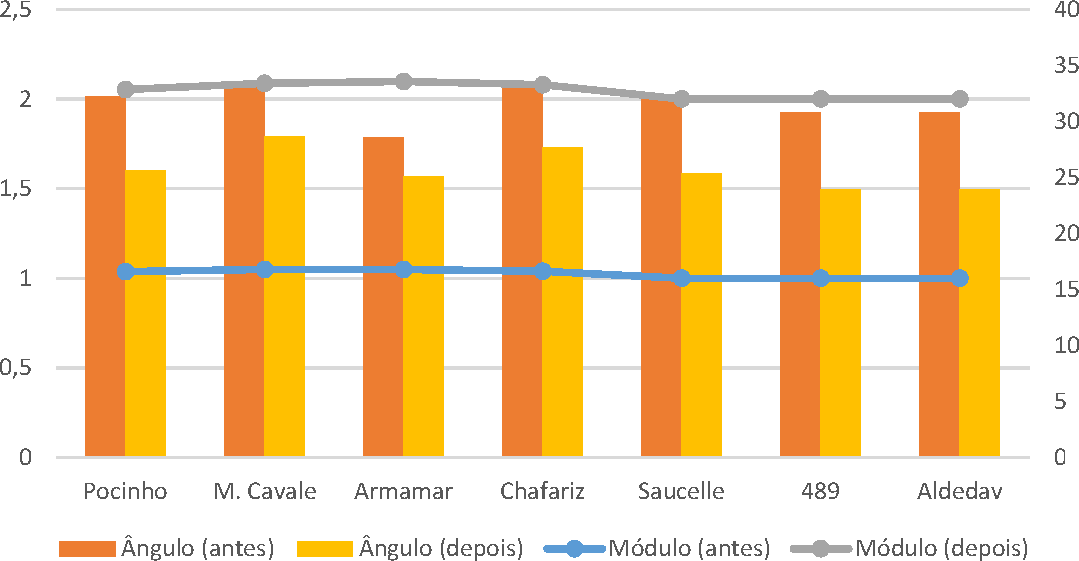
\includegraphics[width=\linewidth]{img/tensoes_barras_caso2.pdf}
	\caption{Análise dos barramentos antes e após o cenário 2}
	\vspace{-3.5mm}
	\caption*{Fonte: autoria própria}
	\label{fig:tensoes_barras_caso2}
\end{figure}

% comentar
\subsubsection{Análise da interligação com a Espanha}
Os impactos da modificação na interligação com a Espanha estão resumidos na Tabela \ref{tab:espanha_caso2}.

\begin{table}[H]
\centering
	\captionsetup{width=0.4\textwidth, font=footnotesize, textfont=bf}
    \begin{tabular}{|
  >{\columncolor[HTML]{000000}}l |c|c|l}
  \cline{1-3}
  {\color[HTML]{FFFFFF} } & \cellcolor[HTML]{000000}{\color[HTML]{FFFFFF} MW} & \cellcolor[HTML]{000000}{\color[HTML]{FFFFFF} MVAr} &  \\ \cline{1-3}
  {\color[HTML]{FFFFFF} Antes}  & 208,9 & 320,5 &  \\ \cline{1-3}
  {\color[HTML]{FFFFFF} Depois} & 207,2 & 104,8 &  \\ \cline{1-3}
  \end{tabular}
  \caption{Interligação com a Espanha antes e após o cenário 2}
  \vspace{-3.5mm}
	\caption*{Fonte: Autoria Própria}
  \label{tab:espanha_caso2}
\end{table}
